\documentclass[pdflatex,sn-basic]{sn-jnl}

        \usepackage{graphicx}
        \usepackage{booktabs}
        \usepackage{array}
        \usepackage{amsmath}
        \usepackage{url}
        \usepackage{hyperref}
        \usepackage{placeins}

        \theoremstyle{thmstyleone}
        \newtheorem{theorem}{Theorem}

        \raggedbottom

        \begin{document}

        \title[AEGIS: Safe LLM-Assisted Natural-Language Analytics]{AEGIS: A Constraint-Based Architecture for Safe LLM-Assisted Natural Language Analytics}

        \author*[1]{\fnm{Md.} \sur{Riaz} \href{https://orcid.org/0009-0003-8850-4122}{(ORCID: 0009-0003-8850-4122)}}\email{mdriaz.wd@gmail.com}

        \affil*[1]{\orgdiv{Department of Computer Science and Engineering}, \orgname{Pundra University of Science and Technology}, \orgaddress{\city{Bogura}, \country{Bangladesh}}}

        \abstract{Natural-language analytics can make relational business data usable for non-technical users, but direct text-to-SQL generation remains hard to control in operational reporting environments. A syntactically valid query can still violate business definitions, expose unauthorized data, or produce an unsafe report artifact. This paper presents AEGIS, a constraint-based architecture for safe LLM-assisted natural-language analytics. AEGIS restricts the language model to typed intent extraction over an approved semantic layer; deterministic components then validate that structured intent, perform query planning, compile SQL from templates, check the compiled query, select a visualization, and persist a reusable widget. The approach is evaluated on a nopCommerce e-commerce deployment using two static reproducible artifacts: a 500-question natural-language benchmark with 425 supported and 75 realistic boundary requests, and nopCommerce's own twenty standard admin reports, whose shipped implementations serve as an independent oracle. On the 500-question benchmark, AEGIS parses 499/500 prompts, answers 423/425 supported requests and executes 422 (99.3\%), and declines 72/75 boundary requests (96.0\%). Against the platform's own report logic on a shared database, fifteen of twenty result sets match exactly; the other five agree on every value and differ only in row count and label column. The same model asked to write SQL directly, with no semantic layer, executes 365/425 supported requests (85.9\%) but answers 25 of the 75 unanswerable questions anyway (33.3\%) and emits two queries containing forbidden constructs. Intent extraction dominates latency at a 9.0 s median, while every deterministic stage after it completes in 3.6 ms. The results show that AEGIS is not an unrestricted natural-language-to-SQL engine. It is a bounded architecture for safe, reusable analytics over an explicitly approved semantic layer.}

        \keywords{natural language interfaces \sep text-to-SQL \sep semantic layer \sep dashboard generation \sep LLM safety \sep business intelligence \sep constrained query generation}

        \maketitle

        \textbf{Md. Riaz} Pundra University of Science and Technology, Bogura, Bangladesh


Natural-language analytics can make relational business data usable for non-technical users, but direct text-to-SQL generation remains hard to control in operational reporting environments. A syntactically valid query can still violate business definitions, expose unauthorized data, or produce an unsafe report artifact. This paper presents AEGIS, a constraint-based architecture for safe LLM-assisted natural-language analytics. AEGIS restricts the language model to typed intent extraction over an approved semantic layer; deterministic components then validate that structured intent, perform query planning, compile SQL from templates, check the compiled query, select a visualization, and persist a reusable widget. The approach is evaluated on a nopCommerce e-commerce deployment using two static reproducible artifacts: a 500-question natural-language benchmark with 425 supported and 75 realistic boundary requests, and nopCommerce's own twenty standard admin reports, whose shipped implementations serve as an independent oracle. On the 500-question benchmark, AEGIS parses 499/500 prompts, answers 423/425 supported requests and executes 422 (99.3\%), and declines 72/75 boundary requests (96.0\%). Against the platform's own report logic on a shared database, fifteen of twenty result sets match exactly; the other five agree on every value and differ only in row count and label column. The same model asked to write SQL directly, with no semantic layer, executes 365/425 supported requests (85.9\%) but answers 25 of the 75 unanswerable questions anyway (33.3\%) and emits two queries containing forbidden constructs. Intent extraction dominates latency at a 9.0 s median, while every deterministic stage after it completes in 3.6 ms. The results show that AEGIS is not an unrestricted natural-language-to-SQL engine. It is a bounded architecture for safe, reusable analytics over an explicitly approved semantic layer.


\section{Introduction}

Organizations store much of their operational knowledge in relational databases: sales transactions, customer records, inventory, payments, shipments, refunds, and similar business data. Although this data is valuable for decision-making, access to it is uneven. Technical users can write SQL queries directly, while non-technical users often depend on developers, analysts, or administrators to prepare reports for them. This creates delay and also discourages repeated exploratory questions such as changing a date range, comparing another product group, or viewing the same metric by a different dimension.


Natural language interfaces to databases (NLIDBs) address this problem by allowing users to ask questions in ordinary language. Recent neural text-to-SQL systems and large language models have improved substantially on benchmark datasets, but practical reporting systems require more than producing a plausible SQL query. In an operational dashboard, the answer must respect business definitions, database permissions, safety constraints, and presentation requirements. A generated query that is syntactically valid can still be unsafe, semantically wrong, or unsuitable for reuse.


This paper presents \textbf{AEGIS} (Analytics Engine with Guaranteed Injection Safety), a constraint-based architecture for safer natural-language analytics. AEGIS does not ask the language model to generate SQL. Instead, the model extracts a structured analytical intent from the user's request. The rest of the pipeline maps that intent to an approved semantic layer, compiles SQL from deterministic templates, validates the query, executes it, selects a visualization, and stores the result as a reusable dashboard widget.


The central idea is to separate language understanding from query execution. The language model is useful for interpreting user wording, but it is not trusted with database structure, SQL syntax, access control, or business definitions. Those responsibilities remain in explicit system components controlled by the application owner. If a request cannot be expressed using the approved semantic layer, AEGIS returns a clarification or rejection rather than substituting the nearest available metric and silently producing a wrong answer.


This work contributes:


\begin{enumerate}
\item A reporting-oriented architecture that converts natural-language requests into persistent dashboard widgets rather than one-off SQL query results.
\item An approved semantic-layer contract for declaring metrics, dimensions, joins, filters, time rules, permissions, and visualization defaults.
\item A deterministic SQL compilation pipeline that generates read-only queries from approved analytical templates instead of model-authored SQL.
\item A grounding and structured-intent validation mechanism that separates answerable requests from unsupported or ambiguous requests before query compilation.
\item A reproducible nopCommerce evaluation protocol combining broad natural-language requests, Admin-oracle fidelity checks, paraphrase robustness, and semantic-coverage tests.
\item Empirical evidence that a bounded semantic-layer system can provide high supported-request execution while preserving explicit rejection behavior for realistic out-of-boundary questions.
\end{enumerate}

The paper is organized as follows. Section 2 reviews related work in natural-language interfaces, text-to-SQL, natural-language visualization, dashboard generation, and semantic layers. Section 3 presents the analytical task taxonomy that motivates the template library. Section 4 presents the AEGIS architecture. Section 5 describes the prototype implementation. Section 6 reports the evaluation. Sections 7-9 discuss implications, limitations, and conclusions.


\section{Related Work}

\subsection{Natural Language Interfaces to Databases}

Natural language database interfaces have been studied for over four decades. Early systems such as LUNAR (Woods, 1973) and TEAM (Grosz, 1983) used hand-crafted grammars and domain-specific ontologies to parse queries. These systems were brittle under vocabulary variation but established the core insight that query understanding requires a bridge between natural language and schema semantics.


NaLIR \citep{li2014nalir} is an important modern NLIDB because it treats ambiguity as a real problem to solve rather than an error. By showing users different possible interpretations of their question, NaLIR improves accuracy but requires the user to actively participate. AEGIS uses a similar approach - asking for clarification when the meaning is unclear - but extends it into a full widget lifecycle that NaLIR does not cover. Survey work (\citep{affolter2019survey}; \citep{liu2026review}) confirms that ambiguity, portability, schema complexity, and controlled access remain ongoing challenges across NLIDB generations and are not solved by bigger models alone.


\subsection{Neural Text-to-SQL and Benchmark Progress}

Seq2SQL and WikiSQL moved the field toward neural approaches \citep{zhong2018seq2sql}, which showed that aligned training data could teach models to produce SQL. Spider \citep{yu2018spider} advanced the challenge significantly by introducing cross-domain schemas and complex multi-table queries, becoming the standard benchmark. SParC and CoSQL \citep{yu2019sparc,yu2019cosql} extended the evaluation to conversational and contextual settings. BIRD \citep{li2023bird} brought benchmark queries closer to production conditions by emphasizing large databases, value grounding, and query efficiency.


Schema-aware encoding, introduced in RAT-SQL \citep{wang2020ratsql}, showed that explicitly modeling schema relationships improves accuracy on new databases. Constrained decoding approaches such as PICARD \citep{scholak2021picard} showed that rejecting invalid SQL tokens during generation improves results. More recent systems like G-SQL \citep{shalaan2025gsql} and TriSQL \citep{su2026robust} add rule guidance and multi-stage checking. These systems improve text-to-SQL accuracy, but they still focus on SQL generation. They do not address safe data access, permission control, widget storage, or chart selection, which are the concerns AEGIS targets.


\subsection{Natural Language for Visualization}

A parallel research stream focuses on NL-driven chart generation rather than SQL generation. nl4dv \citep{narechania2021nl4dv} maps natural language queries to analytic tasks and visual encodings. nvBench \citep{luo2021nl2vis} introduced a cross-domain benchmark for NL-to-visualization. Eviza \citep{setlur2016eviza} enabled conversational interaction with existing visualizations. DataTone \citep{gao2015datatone} managed ambiguity in NL visualization interfaces through mixed-initiative interaction, surfacing alternative chart interpretations to users - a concept AEGIS adopts in its clarification model.


\subsection{Dashboard Generation}

Recent work also treats dashboard generation as an automated design problem. DashBot \citep{deng2023dashbot} proposed using deep reinforcement learning to compose dashboards from a set of data insights. MultiVision \citep{wu2022multivision} used bidirectional LSTM models to score individual charts and combine them into multi-view dashboards. DataShot \citep{wang2020datashot} and Calliope \citep{shi2021calliope} used statistical fact extraction followed by template-based layout to generate narrative data documents.


\subsection{Semantic Layers and Controlled Analytics}

A semantic layer is a business-logic abstraction that maps business concepts to the actual database tables and columns. Commercial tools like dbt Metrics, Looker LookML, and Apache Superset implement semantic layers in different ways. Lehmann et al. (2022) stress the importance of controlled data access in practical NL database interfaces. Structured output enforcement for LLMs \citep{openai2024structured} has been shown to improve the reliability of typed object generation, which AEGIS uses for intent extraction. The reviewed work does not use a semantic layer as the main safety mechanism for an LLM-assisted reporting system.


\subsection{Comparative Summary}

\begin{table}[t]
\caption{Comparative positioning of AEGIS against related systems.}
\label{tab:1}
\centering
\scriptsize
\setlength{\tabcolsep}{3pt}
\begin{tabular}{p{0.25\textwidth}ccccccp{0.16\textwidth}}
\toprule
System & NL & Sem. & Safe SQL & Viz. & Widget & Intent Validation & Evaluation \\
\midrule
Spider / BIRD (Yu '18; Li '23) & Yes & - & - & - & - & - & Benchmark \\
Seq2SQL (Zhong '18) & Yes & - & - & - & - & - & Benchmark \\
RAT-SQL (Wang '20) & Yes & - & - & - & - & - & Benchmark \\
PICARD (Scholak '21) & Yes & - & Partial & - & - & - & Benchmark \\
NaLIR (Li '14) & Yes & - & - & - & - & - & Benchmark \\
nl4dv (Narechania '21) & Yes & - & - & Yes & - & - & In-memory \\
DashBot (Deng '23) & - & - & - & Yes & Partial & - & Synthetic \\
Lehmann et al. (2022) & - & Yes & - & - & - & - & Position \\
\textbf{AEGIS (this work)} & \textbf{Yes} & \textbf{Yes} & \textbf{Yes} & \textbf{Yes} & \textbf{Yes} & \textbf{Yes} & \textbf{nopCommerce evaluation} \\
\bottomrule
\end{tabular}
\end{table}

\section{Analytical Task Taxonomy}

\subsection{Taxonomy Construction}

The eleven analytics primitives below were identified through a review of representative e-commerce and administrative reporting requests conducted during AEGIS design. This taxonomy is a design artifact: it defines the finite request shapes the compiler is allowed to render, rather than claiming that all possible user questions fit these shapes.


\begin{table}[t]
\caption{Analytical task taxonomy used by the AEGIS compiler.}
\label{tab:2}
\begin{tabular}{p{0.26\textwidth}p{0.20\textwidth}p{0.20\textwidth}}
\toprule
Pattern & Purpose & Example \\
\midrule
KPI / Aggregate & Single-number business summary & Total revenue this month \\
Ranking & Top or bottom entities by metric & Top products by revenue \\
Exception / Filter & Rows that meet an operational condition & Low-stock products \\
Trend Analysis & Metric over time & Monthly sales trend \\
Comparison & Metric compared across groups or periods & Revenue by order status \\
Summary / Group & Grouped business overview & Orders by payment status \\
Cohort & Population split by lifecycle stage & New versus returning customers \\
Funnel & Stepwise business process & Checkout progression \\
Correlate & Relationship between two measures & Discount versus order value \\
Segment & Breakdown by business dimension & Revenue by country \\
Tabular & Detailed record listing & Latest orders \\
\bottomrule
\end{tabular}
\end{table}

The final evaluation does not use the older mixed general benchmark as the main evidence source. Instead, it uses a static nopCommerce corpus with 500 natural-language questions: 425 supported questions that should be answerable by the implemented semantic layer and 75 realistic e-commerce boundary questions that should be rejected or clarified.


\subsection{Position of the Evaluation Corpus}

The benchmark is finite by design. It measures whether the implemented nopCommerce semantic layer covers useful combinations of approved metrics, dimensions, time rules, predicates, and analytical patterns. It does not measure open-ended text-to-SQL capability. This matches the AEGIS claim: useful natural-language analytics should be broad within the declared semantic layer and explicit outside it.


The 500-question dataset, the extracted semantics of nopCommerce's twenty standard admin reports, and their oracle queries are static artifacts so that the claims can be inspected and rerun.


\section{The AEGIS System}

AEGIS is designed around a simple division of responsibility. The language model interprets the user's wording, but all database-facing behavior is controlled by deterministic system components. This section describes the architecture and the main stages of the pipeline.


\subsection{Design Principles}

AEGIS follows five design principles.


\begin{enumerate}
\item \textbf{Separate understanding from execution.} The LLM is used for intent extraction, not SQL generation.
\item \textbf{Represent business meaning explicitly.} Metrics, dimensions, filters, joins, and time rules are declared in a semantic layer.
\item \textbf{Constrain query construction.} SQL is produced only by deterministic templates over approved semantic-layer objects.
\item \textbf{Treat non-answer as a valid outcome.} Unsupported or ambiguous requests should be rejected or clarified rather than forced into the nearest available query.
\item \textbf{Produce reusable analytical artifacts.} The output is not only a query result, but a dashboard widget with visualization and refresh behavior.
\end{enumerate}

\subsection{System Overview}

\begin{figure}[!htbp]
\centering
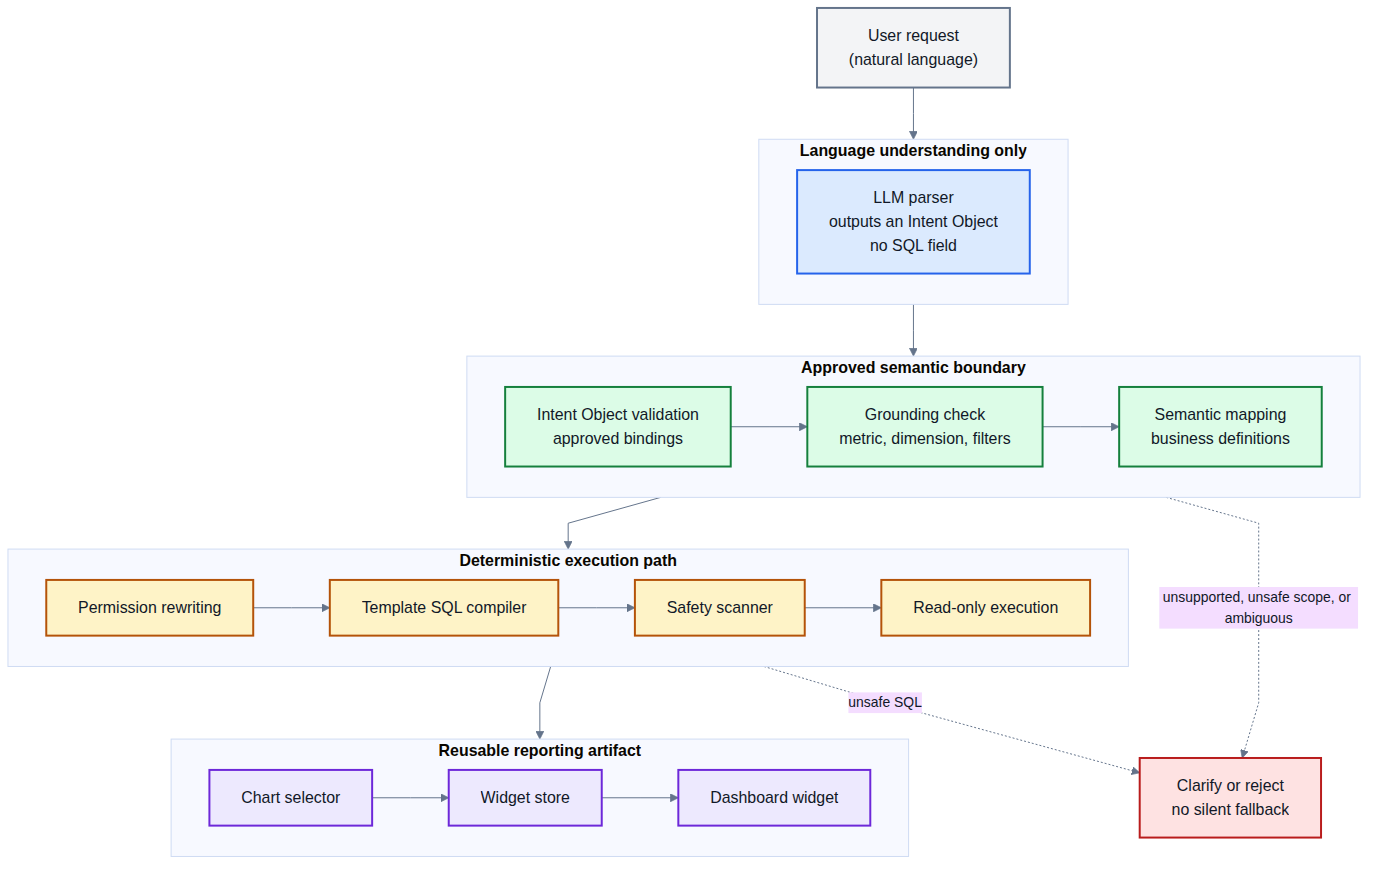
\includegraphics[width=0.88\textwidth]{fig1_architecture_pipeline.png}
\caption{AEGIS architecture pipeline from natural-language request to reusable dashboard widget.}
\label{fig:architecture}
\end{figure}


The pipeline begins with a request such as "Which products brought in the most revenue this month?" The LLM converts the sentence into a structured intent: a ranking request, using the revenue metric, grouped by product, filtered to the current month. AEGIS then checks whether each requested concept is present in the semantic layer. If the concepts are available, the analysis planner builds a canonical plan. If a concept is missing, such as a marketing campaign dimension that has not been modeled, the request is rejected or clarified.


The compiler then converts the plan into SQL using approved templates. The LLM does not choose table names, join clauses, predicates, or SQL syntax. After compilation, a safety scanner verifies that the query is read-only and contains no forbidden constructs. The query is then executed, a visualization is selected, and the result is stored as a reusable widget.


The pipeline is:


\begin{quote}User Request -> LLM Intent Parser -> Structured Intent Validator -> Semantic Mapper -> Analysis Planner -> Safe Query Compiler -> Permission Rewriter -> Query Executor -> Visualization Selector -> Widget Engine -> Dashboard\end{quote}

This staged design separates AEGIS from direct LLM-to-SQL systems. A direct system asks the model to produce executable SQL; AEGIS asks the model only to describe the user's analytical intent.



\begin{figure}[!htbp]
\centering
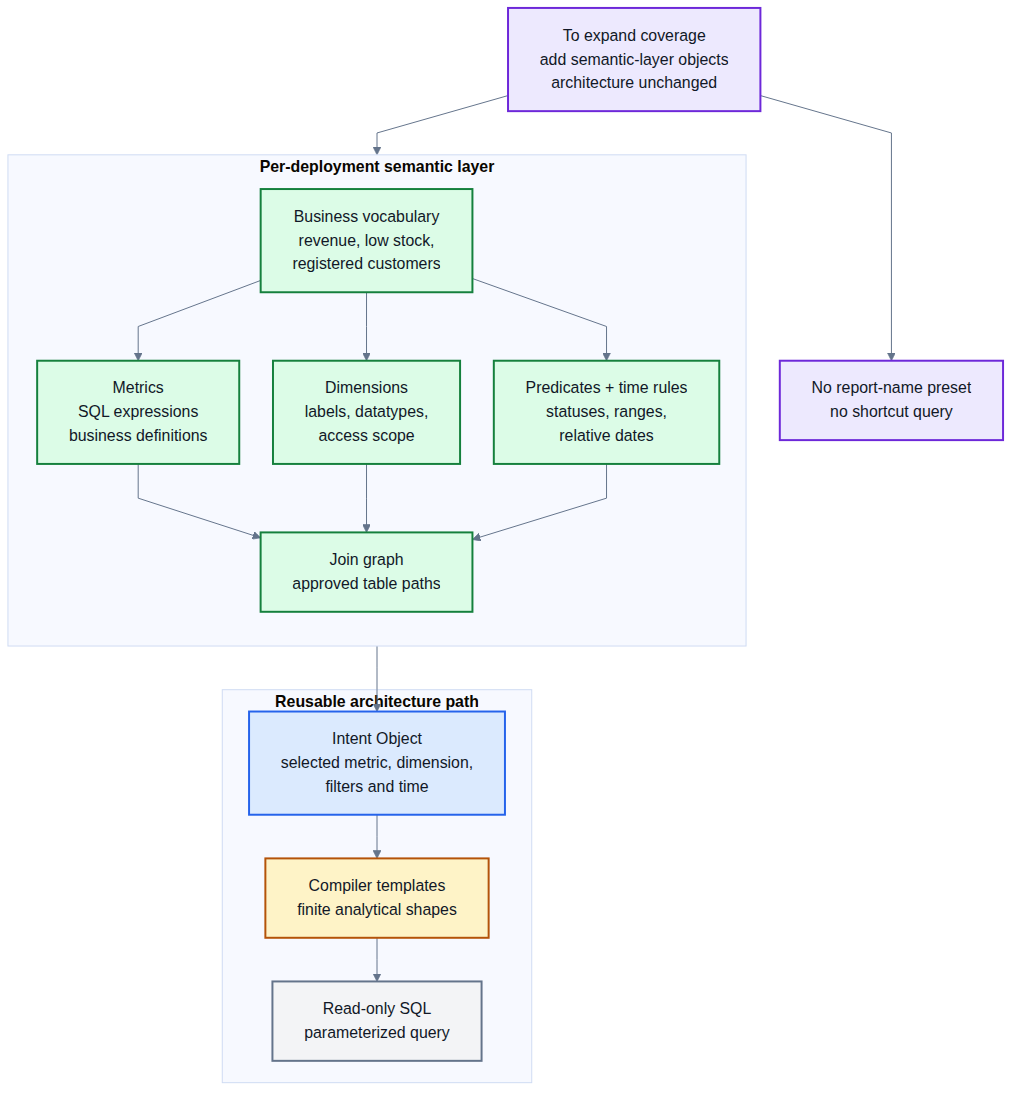
\includegraphics[width=0.82\textwidth]{fig2_semantic_layer.png}
\caption{Semantic-layer modularity: Approved business concepts are composed before SQL is compiled.}
\label{fig:semantic}
\end{figure}

\subsection{Semantic Layer}

The semantic layer is the main control point in AEGIS. It defines the business concepts that the system is allowed to answer. A metric specifies a measurable quantity such as revenue, order count, refund amount, or customer count. A dimension specifies how a result can be grouped or filtered, such as product, category, country, order status, payment status, or month. The semantic layer also records required joins, mandatory predicates, access rules, and default visualization choices.


This layer separates business language from the physical database schema. A user may ask for "sales", "amount spent", or "revenue", but the system maps those expressions to one approved metric definition. The same mechanism prevents unsupported concepts from being silently substituted. If the semantic layer does not define campaign attribution, review sentiment, or forecasted demand, AEGIS should not invent a query for those concepts.


\subsection{Intent Parsing with Vocabulary Injection}

AEGIS builds the LLM prompt from the semantic layer at runtime. The prompt lists the approved metrics and dimensions with short descriptions, and instructs the model to return a typed JSON intent object. This is called vocabulary injection. It allows the model to map flexible user wording onto approved identifiers without maintaining a separate synonym dictionary.


The parser output contains fields such as the analytical pattern, metric, dimension, time phrase, filters, sort order, and limit. For example, a request for "top products by revenue this month" should produce a ranking intent with \texttt{revenue} as the metric, \texttt{product\_name} as the dimension, descending sort order, and a current-month time rule. The parser does not produce SQL.


\subsection{Grounding and Structured Intent Validation}

The grounding stage verifies that each parsed term corresponds to an approved semantic object. It returns one of three outcomes for each important slot: resolved, ambiguous, or unsupported. This prevents silent fallback from one business concept to another.


AEGIS validates the structured intent produced by the LLM against approved metrics, dimensions, filters, analytical patterns, and join rules. The original request text is not treated as a broad vocabulary checklist, because vague and multilingual wording is exactly what the LLM is meant to normalize. Raw text is retained only for narrow non-executable cues: destructive write requests, direct credential or secret requests, and explicit prediction, causal explanation, or sentiment-analysis requests outside the SQL-only prototype scope. If the LLM misinterprets vague unsupported language as a supported intent, that remains an intent-extraction limitation mitigated by confidence, clarification, and visible debug traces; the deterministic compiler can only guarantee that any executed SQL comes from approved semantic definitions.


\subsection{Time Grammar and Analysis Planning}

Time expressions are normalized by a dedicated time grammar. Phrases such as "today", "this month", "last 30 days", and "monthly" are converted into explicit time rules. Unsupported time phrases are reported rather than ignored. This avoids a common reporting error in which a time filter is dropped and the query silently runs over all available data.


After grounding and time normalization, AEGIS builds an analysis plan. The plan records the approved metric, dimension, filters, time rule, visualization pattern, sort order, and limit. This plan is the contract between natural-language interpretation and deterministic query compilation.



\begin{figure}[!htbp]
\centering
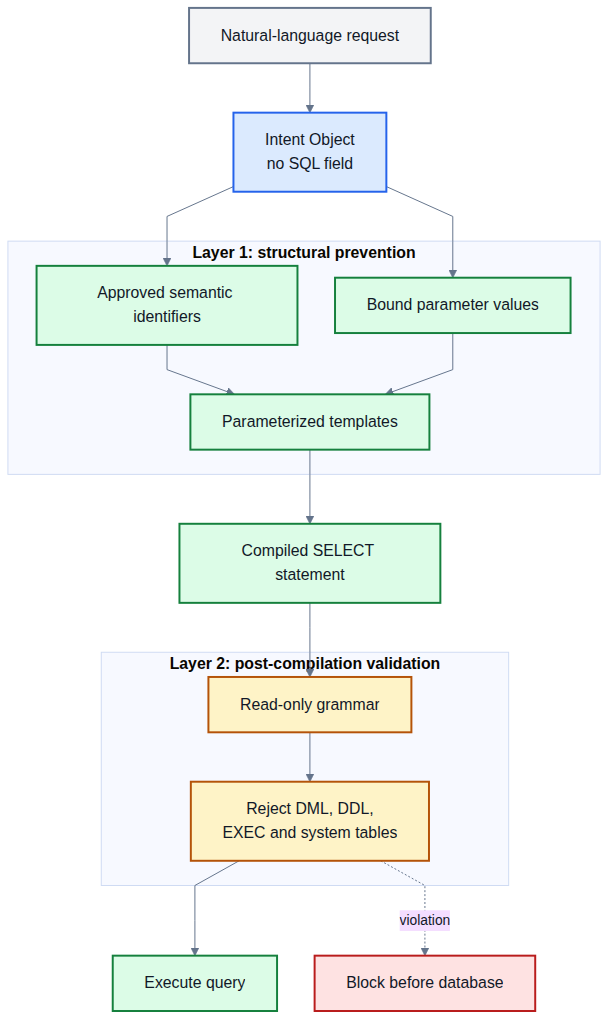
\includegraphics[width=0.78\textwidth]{fig3_sql_safety.png}
\caption{Two-layer SQL safety model combining structural prevention with post-compilation validation.}
\label{fig:safety}
\end{figure}

\subsection{Safe Query Compiler}

The compiler converts an analysis plan into SQL by expanding approved templates. It selects the required tables, resolves join paths from the semantic-layer graph, applies mandatory predicates such as soft-delete filters, binds user values as parameters, and adds grouping, ordering, and limits according to the analytical pattern.


The compiler also handles reporting-specific correctness rules. For example, an order-level metric such as total revenue cannot be grouped directly by product category without double-counting orders that contain multiple line items. In such cases, the semantic layer can define an item-grain equivalent metric, and the planner can use that safer definition for product-level breakdowns.


The compiled SQL is then checked by a post-compilation safety scanner. Queries containing write operations, system-table access, or other forbidden constructs are rejected. The safety guarantee depends on the fact that SQL structure comes from templates and semantic-layer definitions, not from untrusted natural-language text.



\begin{figure}[!htbp]
\centering
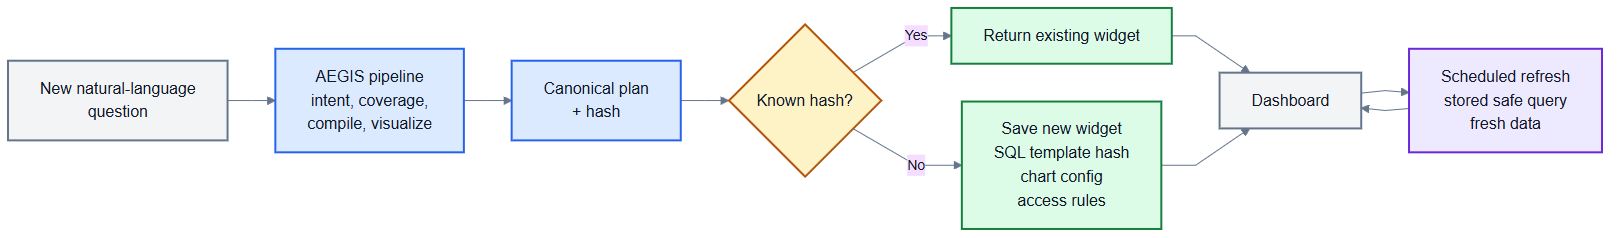
\includegraphics[width=0.78\textwidth]{fig4_widget_lifecycle.png}
\caption{Widget lifecycle for reusable natural-language analytics.}
\label{fig:widget}
\end{figure}

\subsection{Visualization and Widget Generation}

Once a query executes, AEGIS selects a visualization based on the analytical pattern and result shape. Scalar results become KPI cards, ranked lists become bar charts or tables, trends become line charts, and tabular results remain tables. The widget engine stores the generated artifact so that users can refresh and reuse the report rather than asking the same question repeatedly.


\subsection{Terminal Outcomes}

AEGIS has three terminal outcomes:


\begin{itemize}
\item \textbf{ANSWER:} the request is supported, SQL is compiled, and a widget is produced.
\item \textbf{CLARIFY:} the request is potentially answerable but ambiguous, so the system asks a specific follow-up question.
\item \textbf{REJECT:} the request depends on concepts or operations outside the approved semantic layer.
\end{itemize}

This explicit outcome model matters because it keeps unsupported requests visible. A refusal is not treated as a crash or a missing feature when the request is genuinely outside scope; it is the correct behavior for a bounded analytical system.


\section{Implementation}

AEGIS is implemented as a web application with a vanilla HTML/JavaScript frontend (jQuery, Chart.js) and a Python (FastAPI) backend targeting a production nopCommerce 4.70 schema.


\begin{itemize}
\item \textbf{LLM Integration:} An LLM API exposed through an OpenAI-compatible \texttt{/v1/chat/completions} interface, reached through the \texttt{CUSTOM} provider profile in \texttt{aegis/server/ai\_config.py} whenever \texttt{LLM\_BASE\_URL} is set, with \texttt{LLM\_MODEL} naming the model to request. AEGIS uses structured JSON output enforcement and a system prompt constructed by injecting approved metric and dimension IDs. The reported evaluation used this OpenAI-compatible LLM API; the SQL compiler and safety layer are independent of the provider because they consume only the typed intent object.
\item \textbf{Rate Limiting:} Provider-agnostic configuration module (\texttt{ai\_config.py}) with sliding-window rate limiter and concurrency-safe \texttt{asyncio.Lock}.
\item \textbf{Semantic Layer:} Python configuration modules containing the approved nopCommerce metrics, dimensions, predicates, and join paths used by the static evaluation corpus. The implementation deliberately keeps synonyms out of a separate hand-maintained dictionary; wording coverage is handled through dynamic vocabulary injection over semantic-layer descriptions.
\item \textbf{SQL Compiler:} Parameterized MySQL templates. BFS join path resolution across 14 tables (12 aliases). Post-compilation \texttt{\_validate\_sql\_safety()} checks 16 forbidden patterns.
\item \textbf{Visualization Selector:} Rule-based Python dictionaries. Additional rules after data: bar charts with >20 categories become tables, pie charts with >8 slices become bar charts.
\item \textbf{Widget Engine:} SHA-256 plan hash deduplication. JSON file storage in prototype (designed for relational database in production).
\item \textbf{Structured Intent Validator:} Pre-compilation gate rejects unsupported or ambiguous structured metric/dimension/filter bindings, and declines narrow raw-text safety/scope cues such as writes, direct secrets, and explicit non-SQL analytics modes.
\item \textbf{Permission Enforcement:} Permission Rewriter appends role-based WHERE predicates. Five roles: \texttt{public}, \texttt{store\_manager}, \texttt{regional\_manager}, \texttt{read\_only}, \texttt{analyst}.
\end{itemize}

\FloatBarrier
\section{Evaluation}

This section evaluates AEGIS on the nopCommerce e-commerce deployment using static, reproducible datasets. The evaluation separates three concerns that natural-language analytics papers often mix: broad request coverage over the implemented semantic layer, fidelity to first-party reporting semantics where source-derived oracles exist, and correct refusal of plausible requests outside the declared semantic boundary.


\subsection{Evaluation Scope and Reproducibility}

The study uses one production-style schema, nopCommerce. It does not claim that AEGIS is an open-ended text-to-SQL system or that it can answer every possible e-commerce question. The tested claim is narrower: when the required business concepts are declared in the semantic layer and the required result shape is supported by deterministic compiler templates, AEGIS should parse the request, resolve it to approved concepts, compile safe SQL, execute the query, and produce an appropriate report. When a request depends on concepts outside that boundary, the correct behavior is to decline or ask for clarification rather than invent an answer.


All reported figures are backed by static datasets, benchmark scripts, and recorded result files. This matters because the evaluation includes both answerable and intentionally unsupported questions; the same corpus can be inspected and rerun rather than relying on selected examples.


\subsection{Dataset and Environment}

All executable evaluations run against the nopCommerce MySQL database seeded from the repository schema and mock data. The loaded database contains 1,200 customers, 2,500 orders, 6,320 order items, 1,492 shipments, 17 products, 8 categories, 8 manufacturers, and 1 store. Date-sensitive tests use the repository date-refresh script so relative phrases such as "today", "this week", and "this month" remain meaningful when the benchmark is rerun.


The evaluation corpus has two static components:


\begin{table}[t]
\caption{Evaluation corpus components.}
\label{tab:3}
\begin{tabular}{p{0.26\textwidth}p{0.20\textwidth}p{0.20\textwidth}}
\toprule
Component & Size & Role \\
\midrule
Natural user questions & 500 & Breadth: 425 answerable questions and 75 realistic e-commerce boundary questions that should be declined. \\
nopCommerce standard admin reports & 20 & Fidelity: the platform's own admin report list, with the platform's own report implementations as the oracle. \\
\bottomrule
\end{tabular}
\end{table}

The two components differ in who chose them. The 500 questions were written for this study, so they measure how the architecture behaves across the range of language a store owner uses. The 20 reports were not: the list is nopCommerce's own admin menu and the comparison target is nopCommerce's own service-layer code, read from source at commit \texttt{64bdf2ff08c8b39e65717bcf974fb43dc2ef68f2} (version 5.00.0). Comparing against a platform's shipped implementation is stronger evidence than comparing against an expected-answer set written by the same authors as the system under test, because the latter tends to agree with the implementation wherever both authors reasoned the same way.


For reproducibility, the released artifact includes the question set, the report semantics and oracle queries, and the recorded output of every benchmark run under the evaluation artifact directory.


The 500-question dataset's 425 supported questions cover KPI, ranking, trend, segmentation, listing, time-filtered requests, item-grain substitutions, customer/order/product/geography/store/status/payment/shipping dimensions, and approved predicates such as low stock. Its 75 boundary questions remain e-commerce related but require concepts not currently modeled, such as web telemetry, marketing attribution, support tickets, review-text sentiment, forecasting, churn prediction, supplier performance, fraud scoring, delivery SLA analysis, and product affinity.


Intent extraction was served by an OpenAI-compatible gateway configured with a routing alias. The alias resolved to \texttt{gpt-5.5} for 352 of the 500 requests and to \texttt{deepseek-v4-flash} for 147; each result row records the model that actually served it. The run is therefore not pinned to a single model, and figures that depend on parser behaviour should be read with that in mind.


\subsection{Evaluation A: 500-Question Live Natural-Language Benchmark}

The live benchmark sends each of the 500 static natural-language prompts through the AEGIS parser, semantic resolver, deterministic compiler, and MySQL execution path. Intent annotations are used for strict parser-slot comparison only; behavioral success is measured by whether supported questions are answered and executed and whether boundary questions are rejected or clarified.


\begin{table}[t]
\caption{500-question live natural-language benchmark results.}
\label{tab:4}
\begin{tabular}{p{0.26\textwidth}p{0.20\textwidth}}
\toprule
Metric & Result \\
\midrule
Parser success & 499/500 (99.8\%) \\
Supported intent exact match & 313/425 (73.6\%) \\
Supported answer rate & 423/425 (99.5\%) \\
Supported execution validity & 422/425 (99.3\%) \\
Boundary rejection accuracy & 72/75 (96.0\%) \\
\bottomrule
\end{tabular}
\end{table}

An initial pass of this benchmark lost 29 questions to a consecutive block of HTTP 502 responses from the gateway, which reduced the supported answer rate to 92.9\%. Those 29 were retried and 28 answered on the second attempt. Both passes are recorded: the first is what the corpus looks like through a degraded provider, and reporting only the second would present a provider outage as though it never happened, while reporting only the first would attribute that outage to the architecture.


The exact-intent score is intentionally stricter than the behavioral measures. It requires the parser to match the annotation for class, metric, dimension, time phrase, filters, sorting, and limit. A previous run of the same corpus scored 81.2\% on this measure against 73.6\% here; the difference tracks the model mix described above rather than any change to the pipeline.


Two supported questions were refused. Both ask to break refunds down by payment method without naming a measure, and a segment report cannot be constructed without one. Choosing a measure on the requester's behalf is precisely the substitution the resolver is built to avoid, so these are correct refusals rather than failures.


Three boundary questions were answered rather than declined. One was a malformed model reply, which is a parse failure counted here as a boundary miss rather than a decision the system made. The other two are the same question phrased twice, asking to compare two named shipping carriers: the model reported both carrier names in \texttt{unmapped\_terms} and the resolver answered by shipping method regardless. That behaviour is deliberate — a model-reported gap is treated as evidence rather than a verdict, because treating it as a verdict produced a high rate of false refusals — and these two questions are what that setting costs.


The same corpus is also executed with the model removed from the loop, by feeding each question's committed intent annotation directly to the resolver. That configuration resolves, compiles, and executes 425 of 425 supported questions and labels 75 of 75 boundary questions correctly. It is reported here only as a regression gate on the resolver and compiler; because no model participates, it is not an end-to-end result and must not be read as one.


\subsection{Evaluation B: Fidelity Against nopCommerce's Own Report Logic}

Each of nopCommerce's twenty standard admin reports is requested in ordinary business phrasing. Two checks are applied. The first asks whether the request reaches an answer and compiles to SQL. The second executes that SQL and the platform's own query against the same seeded database and compares the returned rows.


\begin{table}[t]
\caption{Fidelity against nopCommerce's own report implementations.}
\label{tab:5}
\begin{tabular}{p{0.26\textwidth}p{0.20\textwidth}}
\toprule
Check & Result \\
\midrule
Reached an answer and compiled to SQL & 20/20 \\
Result set matched the platform's own query & 15/20 (75.0\%) \\
\bottomrule
\end{tabular}
\end{table}

Only the second check tests the claim. The first is satisfied by any query that compiles, and several of these twenty once passed it while being silently wrong — an order-level revenue sum fanned out across item-level joins, a missing soft-delete filter, a customer breakdown grouped by display name. Each returned a plausible, chartable number, so nothing downstream could distinguish it from a correct answer.


The five reports that did not match agree with the platform's query on every value in every overlapping row. Four differ in result-set size, because the platform's own reports carry their own limits of five, fifteen or one hundred rows; two differ in the label column, returning a customer name where the platform's query labels by email address. No report returned a different value. Aligning the limits would mean adding per-report presets, which is the report-specific special-casing the semantic-layer design exists to avoid.


One portability finding is worth recording for anyone reproducing this: the oracle queries reference table names in lower case while the schema creates them capitalised, so on a case-sensitive server every oracle query fails outright. The differential was run with \texttt{lower\_case\_table\_names=1}.


\subsection{Evaluation C: Direct LLM-to-SQL Baseline}

The same model, through the same gateway, was asked to write MySQL directly for the same 500 questions against the same database, with no semantic layer between the model and the SQL. This isolates the architectural variable: the arms differ only in whether the model authors the query.


\begin{table}[t]
\caption{AEGIS and a direct LLM-to-SQL baseline on the same 500 questions.}
\label{tab:6}
\begin{tabular}{p{0.26\textwidth}p{0.20\textwidth}p{0.20\textwidth}}
\toprule
Metric & AEGIS & Direct LLM-to-SQL \\
\midrule
Supported execution validity & 422/425 (99.3\%) & 365/425 (85.9\%) \\
Out-of-scope questions answered & 3/75 (4.0\%) & 25/75 (33.3\%) \\
Queries containing a forbidden construct & 0 & 2/500 \\
Transport failures & 1/500 & 0/500 \\
\bottomrule
\end{tabular}
\end{table}

The middle row carries the finding. A third of the questions the semantic layer cannot express were answered by the unconstrained model with confident, executable SQL. Asked to forecast next month's sales, it returned a query summing past months, which runs and returns a number and forecasts nothing. Asked which customers are likely to churn, it returned a query counting each customer's past orders. Asked what customers say about delivery speed, it returned raw review rows. Each answer is plausible, chartable, and addresses a different question than the one asked, which is the failure mode the architecture is designed to make structurally unreachable rather than statistically rare.


Two baseline queries contained constructs the compiler forbids, both \texttt{UNION}-based attempts to classify review text by keyword matching.


\subsection{Latency}

Per-stage timings were recorded for every supported question in the live benchmark.


\begin{table}[t]
\caption{Per-stage latency over the supported questions of the live benchmark.}
\label{tab:7}
\begin{tabular}{p{0.26\textwidth}p{0.20\textwidth}p{0.20\textwidth}}
\toprule
Stage & Median & 95th percentile \\
\midrule
Intent extraction (model) & 9,029.89 ms & 19,460.15 ms \\
Semantic resolution & 0.89 ms & 1.25 ms \\
SQL compilation & 0.13 ms & 0.21 ms \\
Database execution & 2.54 ms & 12.87 ms \\
All stages after the model & 3.62 ms & 14.02 ms \\
\bottomrule
\end{tabular}
\end{table}

The split matters more than the totals. Substantially all of the wall clock is the model reading the question; the stages that resolve business concepts, decide the join path, emit SQL, and execute it account for a few milliseconds, and the model has no influence over any of them. The model figure is a property of the gateway used here and would change with the provider. The deterministic figures are properties of the architecture and would follow it to another deployment. The direct baseline's generation stage has a comparable median of 9,154.02 ms, confirming that the constrained pipeline does not pay a latency premium for its safety.


\subsection{Safety Evaluation}

SQL safety is enforced structurally. The LLM never emits SQL. It emits a typed intent object over injected semantic-layer vocabulary; the resolver grounds that object to approved metrics, dimensions, predicates, and time rules; the compiler emits parameterized SQL from deterministic templates; and the post-compilation safety monitor rejects forbidden constructs. The primary safety claim is therefore architectural rather than statistical: untrusted natural-language text is not interpolated into executable SQL identifiers or clauses, and no rate of successful defence is being asserted.


The baseline comparison gives that claim an empirical counterpart. Both arms were scanned with the same forbidden-pattern set, imported from the compiler rather than restated, so neither arm is judged by a more lenient rule. The unconstrained arm produced two queries containing a forbidden construct; the constrained arm produced none, and could not have, because no path exists from an intent object to a query the templates do not generate.


\subsection{Interpretation}

Three conclusions follow. First, on the 500-question corpus, AEGIS answers and executes nearly all supported requests while declining the large majority of realistic out-of-boundary ones. Second, against nopCommerce's own report implementations, three quarters of the twenty reports match exactly and the remainder differ only in row count and label column, with no value discrepancy. Third, the same model without a semantic layer answers a third of the unanswerable questions anyway, which is the behaviour the architecture removes rather than reduces.


The main limitation is scope, and it is a consequence of the design rather than an implementation gap. The semantic layer is finite and deployment-specific. Adding telemetry, campaign attribution, review sentiment, forecasting, or supplier operations would require extending it and, for genuinely new result shapes, the compiler templates. This also places the work outside cross-domain benchmarks such as Spider and BIRD, which test generalisation to unseen schemas: a deployment-specific semantic layer does not generalise to an unseen schema by construction, and evaluating against those benchmarks would measure a property this architecture does not claim.


A second limitation is that correctness at scale rests on the twenty reports rather than on all 425 supported questions. For the 425, the evidence is that the compiled SQL resolves and executes, not that every returned answer is the intended one. Extending value-level verification to a stratified sample of the corpus is the most useful next measurement.


\section{Discussion}

The evaluation indicates that AEGIS is most useful when the goal is not unrestricted database exploration, but Approved analytical reporting. In this setting, the important requirement is not only whether a system can produce a SQL query, but whether it can produce a query that respects business definitions, permissions, safety constraints, and reusable reporting workflows.


\subsection{Comparison with Direct LLM-to-SQL}

Direct LLM-to-SQL systems ask the model to generate executable SQL from natural language. This can be flexible, but it leaves safety and semantic correctness dependent on model behavior. AEGIS changes the role of the model. The model extracts intent, while SQL is produced by a deterministic compiler over a semantic layer.


\begin{table}[t]
\caption{Structural comparison between direct LLM-to-SQL and AEGIS.}
\label{tab:8}
\begin{tabular}{p{0.26\textwidth}p{0.20\textwidth}p{0.20\textwidth}}
\toprule
Property & Direct LLM-to-SQL & AEGIS \\
\midrule
SQL generation & Model-generated & Template-compiled \\
Schema exposure to LLM & Usually required & Not required \\
Business definitions & Inferred from schema/context & Declared in semantic layer \\
Unsupported requests & May still produce SQL & Clarify or reject \\
Safety control & Prompting and validation & Structural constraint plus validation \\
Output artifact & Query/result & Saved dashboard widget \\
\bottomrule
\end{tabular}
\end{table}

This difference explains the main trade-off. AEGIS gives up unlimited query flexibility in exchange for stronger control over what can be asked, how it is translated, and what is allowed to execute.


\subsection{Role of the Semantic Layer}

The semantic layer is not only a convenience for matching words to columns. It is the boundary of the system's analytical knowledge. If a metric, dimension, or predicate is declared, users can ask for it in many natural phrasings and combine it with other supported concepts. If it is not declared, AEGIS should not invent an answer.


This design is especially important for business reporting because database column names rarely capture the full business meaning of a report. For example, revenue may need to exclude deleted orders, product-level revenue may need item-grain aggregation, and customer reports may require a specific customer identity field. These definitions belong in the semantic layer rather than in ad hoc SQL generated per request.


\subsection{Refusal as a Correct System Behavior}

A central result of this work is that refusal must be measured, not hidden. In a bounded analytics system, some user questions are outside the implemented semantic layer even if they are reasonable business questions. The 500-question benchmark therefore includes realistic e-commerce boundary requests, and AEGIS is evaluated on whether it rejects or clarifies them.


This is different from treating every non-answer as a failure. For AEGIS, answering an unsupported question with a plausible but wrong query is worse than declining it. The explicit ANSWER / CLARIFY / REJECT outcome model is therefore part of the architecture, not only an error-handling feature.


\subsection{Generality of the Architecture}

The prototype is implemented and evaluated on nopCommerce with MySQL, but the architecture is not tied to that particular schema. To apply AEGIS to another system, the developer must define the semantic layer for that system and provide compiler templates for the target SQL dialect. The architecture remains the same: language understanding is separated from Approved query compilation.


The five reports whose result sets differ from the platform's illustrate this point. None differs in value; they differ in how many rows the platform's own report returns and which column it labels rows by. Matching them exactly would mean encoding per-report presets, which trades the generality of the semantic layer for a cosmetic gain.


\section{Limitations and Future Work}

AEGIS is intentionally bounded. Its safety and auditability come from the fact that all answerable concepts must be declared in the semantic layer and all executable SQL must be produced by deterministic compiler templates. The limitations below should therefore be read as explicit boundaries of the current nopCommerce implementation, not as reasons to bypass the architecture with free-form SQL generation.


\begin{itemize}
\item \textbf{Single-domain evaluation.} The final evaluation is over one e-commerce deployment, nopCommerce. The results show that the architecture works in this domain, but they do not prove cross-domain generality. Future work should repeat the same static-dataset process on a second schema such as WooCommerce or a non-commerce operational database.
\item \textbf{Author-generated natural-language data.} The 500-question dataset is static and checkable, but it is still author-generated. A stronger study would collect questions from store owners or administrators, then annotate answerability and expected semantic bindings with at least two independent annotators.
\item \textbf{Finite semantic coverage.} Boundary questions about web telemetry, marketing attribution, support tickets, review-text sentiment, forecasting, churn prediction, supplier performance, fraud scoring, delivery SLA analysis, and product affinity are deliberately outside the current semantic layer. Supporting them requires adding approved metrics, dimensions, predicates, tables, and templates.
\item \textbf{Report fidelity gap.} Fifteen of nopCommerce's twenty standard admin reports match the platform's own result set exactly. The other five agree on every value but differ in row count, because the platform's reports carry their own limits, or in label column. Closing that gap by adding per-report presets would defeat the purpose of the semantic layer.
\item \textbf{Correctness at scale.} Value-level verification covers the twenty reports, not all 425 supported questions; for those the evidence is that the compiled SQL resolves and executes. Extending value-level checking to a stratified sample of the corpus is the most useful next measurement.
\item \textbf{Model pinning.} The gateway used for intent extraction resolved a routing alias per request, so the reported run spans two models. Each result row records the model that served it, but a single-model run is needed before parser-dependent figures can be attributed to one system.
\item \textbf{LLM dependence for intent extraction.} The compiler and safety layer are deterministic, but natural-language intent extraction still depends on the configured LLM API. The live 500-question benchmark records parser success and exact intent agreement, but future work should compare multiple OpenAI-compatible models on the same static dataset.
\item \textbf{Intent misinterpretation boundary.} AEGIS does not claim to perfectly infer intent from vague language. If the LLM converts an unsupported request into a plausible supported intent, deterministic validation may accept the normalized intent because it is now in the semantic-layer vocabulary. This is a prototype intent-extraction limitation, not a licence for free-form SQL: the executed query still comes only from approved semantic definitions.
\item \textbf{Prototype database target.} The evaluated prototype targets nopCommerce on MySQL. This is an implementation and evaluation-scope choice, not an architectural limitation: the same semantic-layer and deterministic-compilation design can support PostgreSQL, SQL Server, or other databases by adding dialect-specific compiler templates and safety rules.
\item \textbf{Widget persistence.} The prototype stores widget metadata in simple local persistence. A production deployment should move the widget registry to a transactional database with migrations, ownership policies, and administrative audit views.
\end{itemize}

\section{Conclusion}

AEGIS is a system for turning plain-English reporting requests into dynamic, refreshable dashboard widgets over relational databases. Its contribution has three parts.


The first is architectural. The LLM is confined to understanding the question; query construction, chart selection, and widget storage are performed by fixed templates and rules downstream of it. Because the compiler emits SQL only by expanding a closed set of templates over a curated semantic layer, and never by interpolating model-produced text, unsafe SQL is excluded by construction rather than filtered after the fact (Section 4.2, Proposition 1). This is the sense in which the design converts a probabilistic property into a structural one.


The second is a pair of mechanisms for the boundary of that vocabulary. Vocabulary injection removes the manually maintained synonym list and lets the model translate flexible user wording into structured semantic-layer intent. AEGIS then validates that structured intent before compilation, while retaining the original text only for narrow non-executable safety/scope cues. The ANSWER / CLARIFY / REJECT channel gives the pipeline somewhere to put the answer "this cannot be expressed here" when the structured intent is unsupported, ambiguous, destructive, sensitive, or outside the SQL-only analytical mode.


The third is evaluative. The final evaluation rests on two static nopCommerce artifacts rather than unsupported headline claims: a 500-question natural-language benchmark and nopCommerce's own twenty standard admin reports. On the live 500-question run, AEGIS answered 423 of 425 supported requests, executed 422, and declined 72 of 75 realistic boundary requests. Against the platform's own report implementations, fifteen of twenty result sets matched exactly and the remaining five differed only in row count and label column, with no value discrepancy. The same model without a semantic layer answered a third of the unanswerable questions anyway and produced two queries containing constructs the compiler forbids, which is the contrast the architecture is meant to produce.


AEGIS is therefore not an infinite natural-language-to-SQL engine. It is a bounded architecture for safe natural-language analytics over an approved semantic layer, suited to environments where data privacy, consistent reporting definitions, auditability, and reusable reporting widgets matter more than unlimited query flexibility.


        \bmhead{Declarations}

        \textbf{Funding} No funding was received for this work.

        \textbf{Conflict of interest} The author declares no conflict of interest.

        \textbf{Data availability} The evaluation datasets and result artifacts are included with the released research repository.

        \textbf{Code availability} The prototype implementation and manuscript artifacts are maintained in the accompanying repository.

        \textbf{Author contribution} Md. Riaz designed the architecture, implemented the prototype, constructed the evaluation datasets, ran the experiments, and wrote the manuscript.

        \bibliography{references}

        \end{document}
